\documentclass[12pt,a4paper]{report}

% Essential Packages
\usepackage[utf8]{inputenc}
\usepackage[margin=1in]{geometry}
\usepackage{amsmath,amssymb,amsfonts}
\usepackage{graphicx}
\usepackage{booktabs}
\usepackage{array}
\usepackage{tabularx}
\usepackage{setspace}
\usepackage{fancyhdr}
\usepackage{titlesec}
\usepackage{microtype}
\usepackage[hyphens]{url}
\usepackage{tikz}
\usetikzlibrary{shapes.geometric, arrows.meta, positioning, fit, calc}
\usepackage[colorlinks=true,linkcolor=blue,citecolor=blue,urlcolor=blue]{hyperref}

% Line Spacing & Formatting
\onehalfspacing
\setlength{\parskip}{0.8em}
\setlength{\parindent}{0pt}

% Chapter and Heading Spacing (Removes excessive top whitespace on Contents and Chapters)
\titleformat{\chapter}[display]
  {\normalfont\huge\bfseries}{\chaptertitlename\ \thechapter}{10pt}{\huge}
\titlespacing*{\chapter}{0pt}{-30pt}{20pt}

% Header and Footer Setup
\pagestyle{fancy}
\fancyhf{}
\fancyhead[L]{\small \nouppercase{\leftmark}}
\fancyhead[R]{\small METRIX -- SIH26036}
\fancyfoot[C]{\thepage}
\renewcommand{\headrulewidth}{0.4pt}
\renewcommand{\footrulewidth}{0.4pt}

\begin{document}

%======================================================================
% TITLE PAGE
%======================================================================
\begin{titlepage}
    \centering
    \vspace*{0.5cm}
    
    {\Huge \textbf{METRIX}}\\[0.4cm]
    {\large \textbf{Online Verification and Digital Certification System\\for Weighing and Measuring Instruments}}\\[0.8cm]
    
    {\large \textit{A Project-I Report Submitted in Partial Fulfilment for the Award of the Degree of}}\\[0.3cm]
    {\Large \textbf{Bachelor of Technology}}\\[0.2cm]
    {\large (VII Semester, Session 2026--27)}\\[0.6cm]
    
    \textbf{Problem Statement ID: SIH26036}\\
    \textit{Smart India Hackathon (SIH 2026)}\\[1.2cm]
    
    \begin{minipage}{0.48\textwidth}
        \begin{flushleft} \large
            \textbf{Supervised By:}\\
            \textbf{Prof. Mamta Garg}\\
            Dean, Department of CSE\\
            JIET, Jodhpur
        \end{flushleft}
    \end{minipage}
    \hfill
    \begin{minipage}{0.48\textwidth}
        \begin{flushright} \large
            \textbf{Submitted By:}\\
            Vidit J Tiwari (23EJICS178)\\
            Tamanna Parveen (23EJICS169)\\
            Vishnu Kant (23EJICS182)\\[0.2cm]
            \small Section: C \textbar{} Group: 7C2
        \end{flushright}
    \end{minipage}
    
    \vfill
    
    \includegraphics[width=0.22\textwidth]{example-image} \\[0.4cm]
    
    {\large \textbf{Department of Computer Science and Engineering}}\\
    {\large \textbf{Jodhpur Institute of Engineering and Technology (Autonomous)}}\\
    {\normalsize Affiliated with Bikaner Technical University}\\
    {\normalsize Jodhpur, Rajasthan, India}\\
    {\normalsize Academic Year 2026--27}
\end{titlepage}

%======================================================================
% TABLE OF CONTENTS
%======================================================================
\newpage
\pagenumbering{roman}
\tableofcontents

%======================================================================
% CHAPTER INCLUSIONS
%======================================================================
\newpage
\pagenumbering{arabic}
\setcounter{page}{1}

%======================================================================
\chapter{Introduction}
%======================================================================

\section{Project Overview}
\textbf{METRIX} is a secure, web-based Online Verification and Digital Certification System developed for Smart India Hackathon (SIH 2026) Problem Statement \textbf{SIH26036} under the Department of Consumer Affairs, Government of India. Under the Legal Metrology Act, 2009, all commercial weighing and measuring instruments must undergo periodic verification by authorized Legal Metrology Officers (LMOs) or Government Approved Test Centres (GATCs). 

METRIX digitizes this end-to-end statutory lifecycle—enabling online instrument registration, digital application submission, field inspection logging against Maximum Permissible Error (MPE) thresholds, tamper-evident digital certificate generation with verifiable QR codes, and automated expiry monitoring.

\section{Problem Statement and Motivation}
Traditional legal metrology verification relies heavily on physical paper ledgers, manual challans, and brass stamping. This causes severe administrative delays, siloed records across districts, certificate counterfeiting, and an absence of consumer-facing verification at the point of sale. METRIX replaces these fragmented manual steps with a unified, transparent digital platform.

\section{Project Objectives}
The primary objectives of the project are:
\begin{enumerate}
    \item \textbf{Online Registration \& Application:} Enable commercial businesses to register instruments and apply for initial and periodic verification online.
    \item \textbf{Inspection Scheduling \& Allocation:} Provide dynamic workload distribution for LMOs and accredited GATCs.
    \item \textbf{Digital Inspection Logging:} Implement standardized digital checklists to record load tests, repeatability, and MPE compliance.
    \item \textbf{Tamper-Evident Certification:} Generate verifiable PDF certificates embedded with dynamic QR codes and SHA-256 integrity hashes.
    \item \textbf{Public Verification Portal:} Provide a zero-login interface for citizens and enforcement officers to verify instrument calibration via QR scan.
    \item \textbf{Compliance \& Expiry Monitoring:} Automatically compute certificate validity and alert custodians prior to statutory expiry.
\end{enumerate}

\section{Scope and Technical Stack}
METRIX is built as a lightweight, modular web application:
\begin{itemize}
    \item \textbf{Frontend:} React.js, Next.js (App Router), TypeScript, Tailwind CSS.
    \item \textbf{Backend:} FastAPI (Python 3.10+), Pydantic v2, SQLAlchemy 2.x.
    \item \textbf{Database:} PostgreSQL relational database.
    \item \textbf{Certificates \& QR:} ReportLab PDF engine and Python \texttt{qrcode}.
\end{itemize}
In accordance with project constraints, the application is developed as a software-only modular monolith without external brokers (Kafka/RabbitMQ), Docker/Kubernetes, or AI/ML components.

%======================================================================
\chapter{Literature Survey}
%======================================================================

\section{Introduction}
Legal metrology enforces statutory standards on commercial weighing and measuring equipment to ensure trade fairness and consumer protection under the Legal Metrology Act, 2009. While traditional enforcement relies on physical lead seals and paper certificates, global standards bodies and national agencies are transitioning toward digital certification systems.

\section{Review of Key Initiatives}
\begin{enumerate}
    \item \textbf{OIML Digital Metrology (2025):} Highlights national initiatives (such as Austria's BEV MMEII portal) that utilize QR-enabled certificates to enable real-time consumer verification of measuring instruments.
    \item \textbf{PTB Digital Calibration Architecture (2024):} Germany's national metrology institute established modular, REST-based frameworks for exchanging structured Digital Calibration Certificates (DCC).
    \item \textbf{India's `e-Maap' Portal (2026):} Launched by the Department of Consumer Affairs to centralize verification and licensing, demonstrating government commitment to digital metrology.
    \item \textbf{Anti-Counterfeit QR Frameworks (2024):} Recent research proves that embedding cryptographic SHA-256 digests and server-bound QR verification endpoints effectively eliminates electronic certificate forgery.
\end{enumerate}

\section{Comparative Evaluation}
Table~\ref{tab:literature_comparison} highlights key distinctions between legacy methods, first-generation portals, and METRIX.

\begin{table}[htbp]
\centering
\small
\caption{Comparison of Verification Approaches}
\label{tab:literature_comparison}
\renewcommand{\arraystretch}{1.15}
\begin{tabular}{|l|p{3.5cm}|p{3.8cm}|p{4.2cm}|}
\hline
\textbf{Feature} & \textbf{Legacy Paper Stamping} & \textbf{First-Gen Portals (e-Maap)} & \textbf{METRIX Platform} \\ \hline
Application & Physical paper forms & Centralized web forms & Guided digital wizard \\ \hline
Inspection & Handwritten sheets & Offline data transcription & Direct digital checklist \\ \hline
Certificate & Physical paper certificate & Static downloadable PDF & Tamper-evident PDF with dynamic QR \\ \hline
Verification & Visual stamp check & Portal search by number & Instant zero-login QR scan \\ \hline
Expiry & Untracked manual ledgers & Generic bulk reminders & Automated lifecycle notifications \\ \hline
\end{tabular}
\end{table}

\section{Research Gap and Solution Motivation}
Existing systems either focus solely on industrial laboratory calibrations or operate as heavy centralized monoliths without lightweight, state-level modular architectures. Furthermore, they lack direct point-of-sale public QR authentication and automated re-verification cycles. 

METRIX resolves these gaps through five integrated pillars: (i) centralized instrument registry, (ii) role-based workflow for officers and test centres, (iii) digital MPE observation logging, (iv) QR-enabled tamper-evident certification, and (v) frictionless public authentication with proactive expiry tracking.

%======================================================================
\chapter{Requirement Specification \& Methodology}
%======================================================================

\section{Software Development Life Cycle (SDLC)}
METRIX is developed using an \textbf{Agile and Iterative Methodology} over a four-week delivery timeline. Given the multi-stakeholder nature of legal metrology, requirements and interfaces are developed and validated in weekly sprint increments:
\begin{itemize}
    \item \textbf{Week 1 (Sprint 1):} Requirement analysis, modular monolith architecture, database schema, and JWT-based authentication with Role-Based Access Control (RBAC).
    \item \textbf{Week 2 (Sprint 2):} Instrument registration catalog, guided verification application wizard, and multi-state application tracking.
    \item \textbf{Week 3 (Sprint 3):} Inspection scheduling, digital MPE observation recording, and ReportLab PDF certificate generation with embedded QR codes.
    \item \textbf{Week 4 (Sprint 4):} Public QR verification portal, automated expiry monitoring, role-specific dashboards, and integration testing.
\end{itemize}

\section{Actor Roles and Use Case Diagram}
The system defines five primary actors:
\begin{itemize}
    \item \textbf{Instrument Owner / Business:} Registers instruments, submits verification applications, uploads payment challans, and tracks certificate status.
    \item \textbf{Legal Metrology Officer (LMO):} Reviews district applications, conducts physical inspections, records error observations, and issues digital certificates.
    \item \textbf{Government Approved Test Centre (GATC):} Receives specialized instrument verification tasks and logs official calibration observations.
    \item \textbf{Administrator:} Oversees user accounts, allocates inspection queues, and monitors district compliance dashboards.
    \item \textbf{Public / Citizen Consumer:} Scans certificate QR codes to verify calibration authenticity in real time without requiring login credentials.
\end{itemize}

\begin{figure}[htbp]
\centering
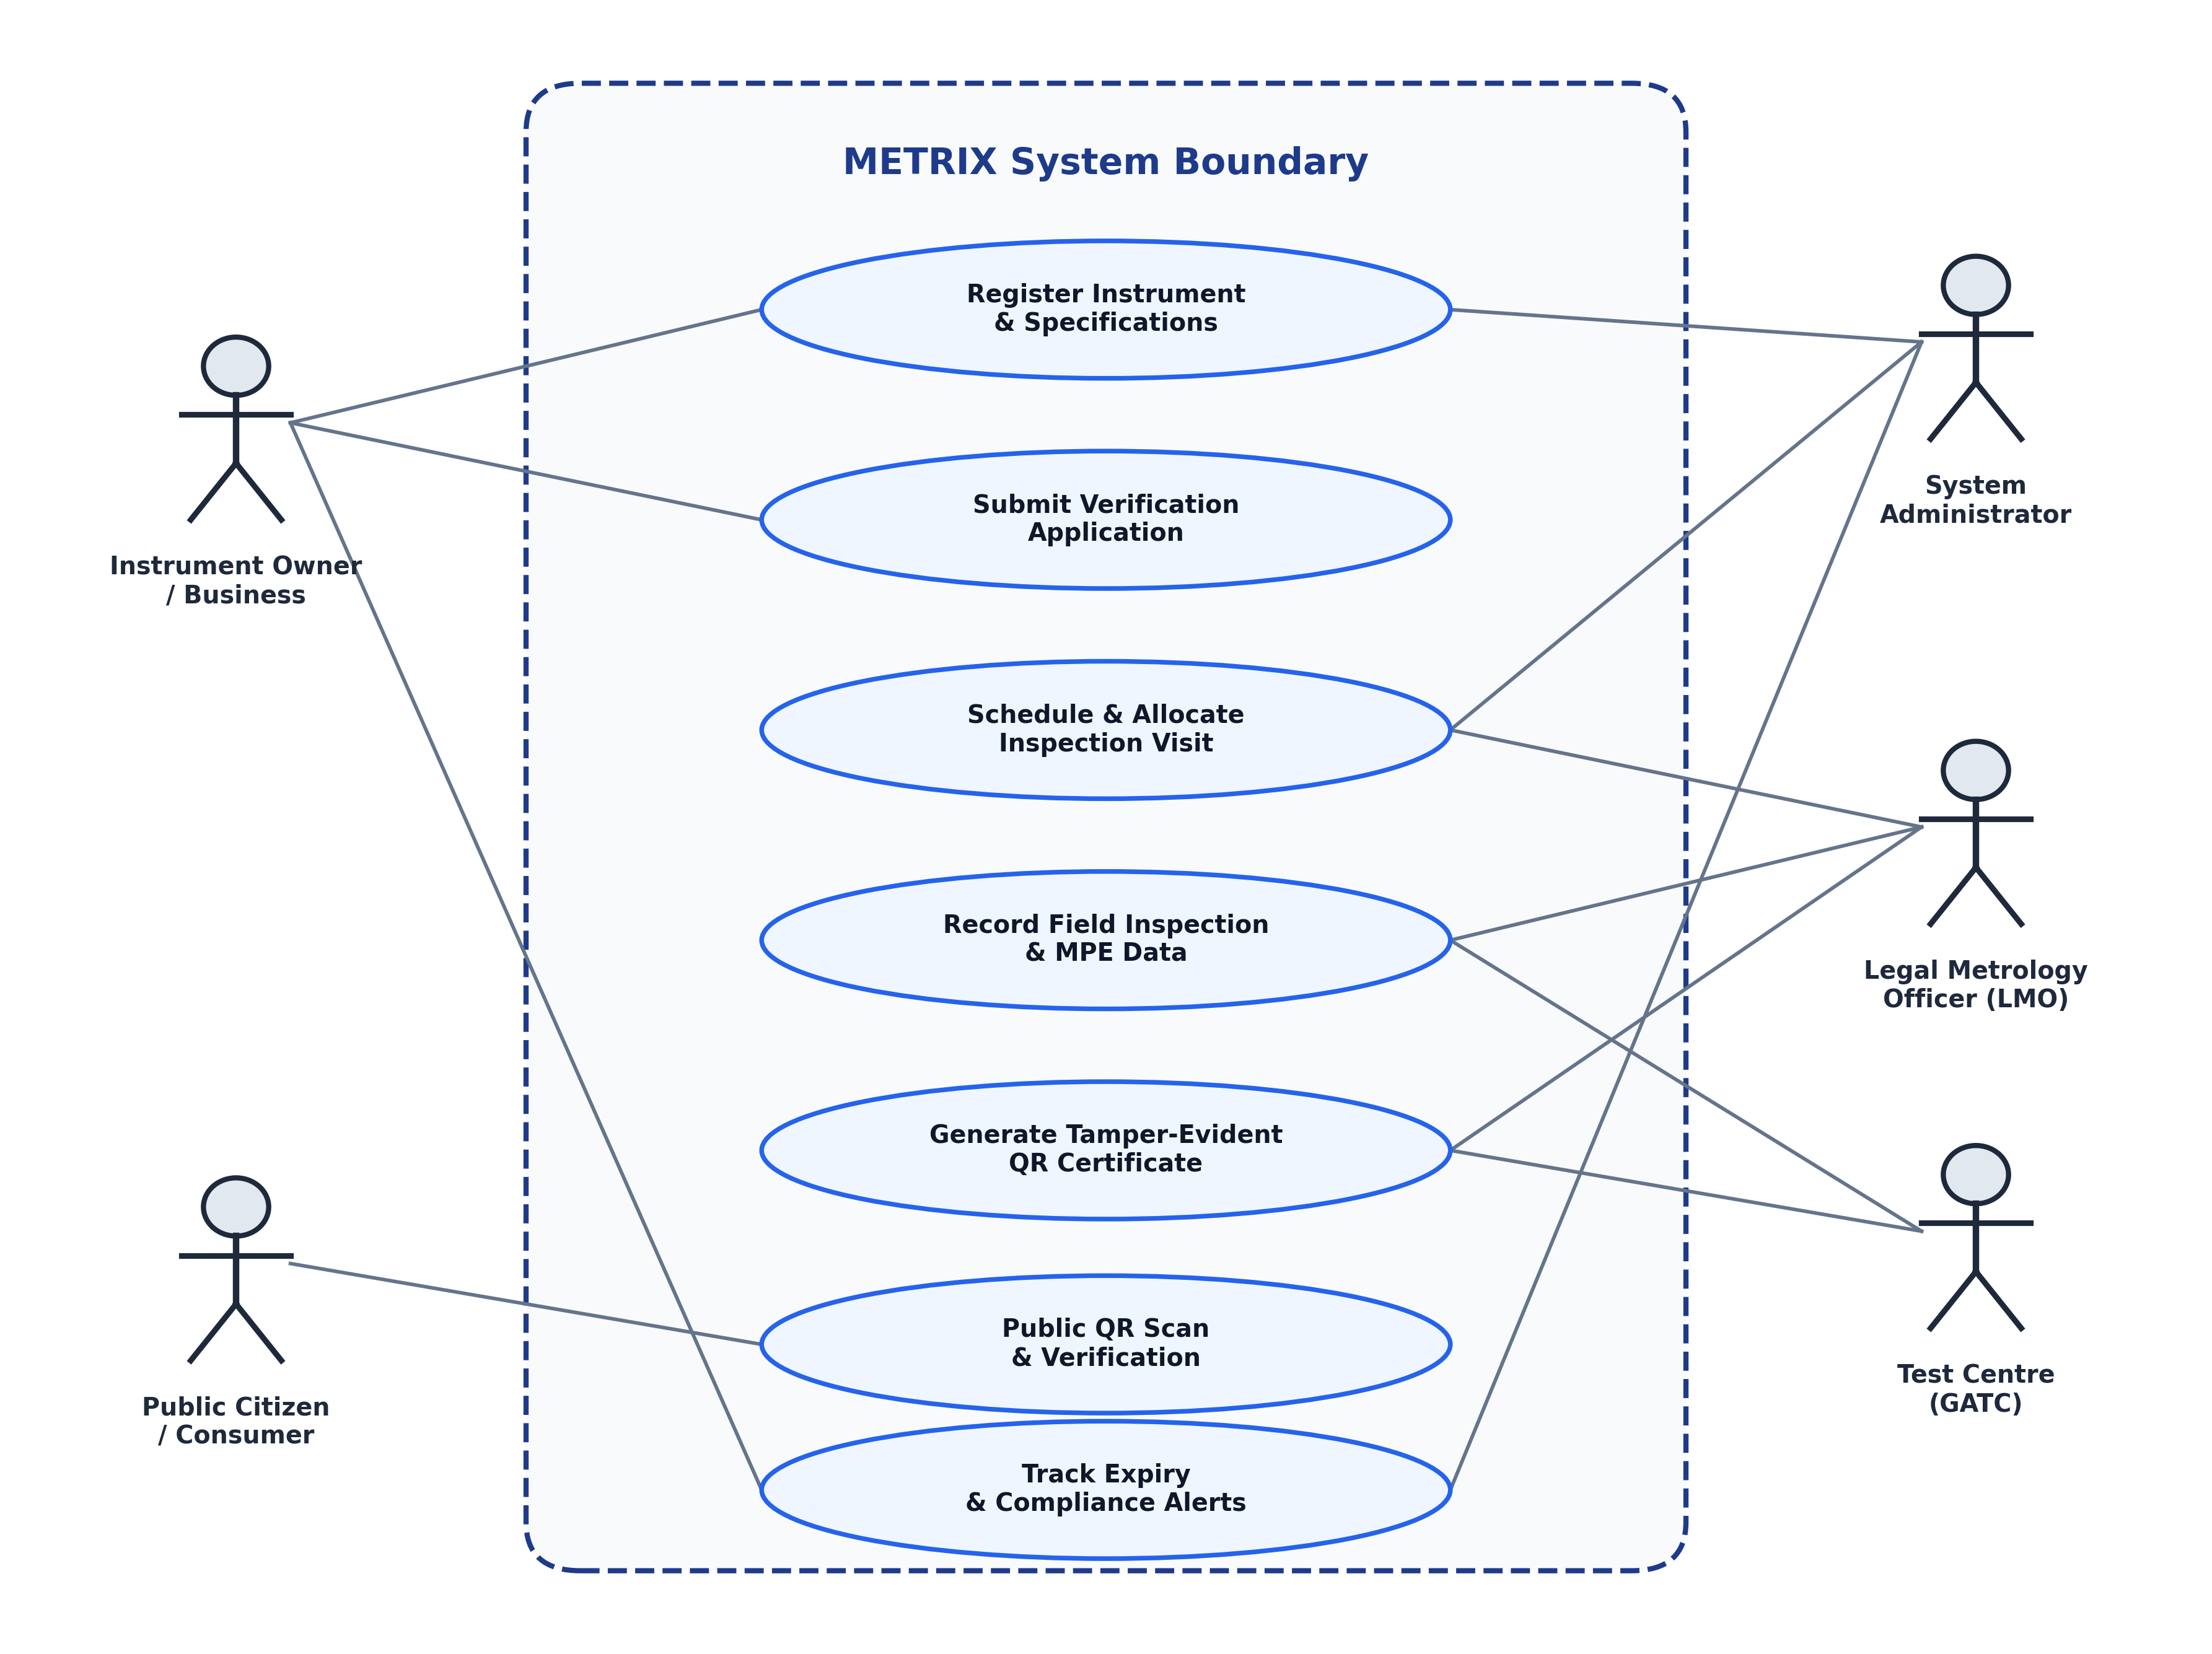
\includegraphics[width=0.95\textwidth]{use_case_diagram.png}
\caption{UML Use Case Diagram of the METRIX System}
\label{fig:use_case_diagram}
\end{figure}

\section{System Interfaces}
\begin{itemize}
    \item \textbf{Software Interfaces:} Next.js (TypeScript, Tailwind CSS) communicating via RESTful JSON APIs with a FastAPI (Python 3.10+) backend, persisting data in PostgreSQL 14+ via SQLAlchemy 2.x ORM. Certificates are generated via ReportLab and Python \texttt{qrcode}.
    \item \textbf{Hardware Interfaces:} Standard desktop, tablet, and mobile browsers, utilizing integrated device cameras for optical QR code scanning.
    \item \textbf{Communication Protocols:} Secure HTTPS/TLS 1.3 transport using JSON data payloads and HTTP \texttt{Authorization: Bearer <JWT>} headers.
\end{itemize}

\section{System Requirements and Constraints}
\begin{itemize}
    \item \textbf{Minimum Hardware:} Dual-Core CPU, 4 GB RAM, 10 GB SSD storage.
    \item \textbf{Software Stack:} Linux / Windows OS, Python 3.10+, Node.js 18+, PostgreSQL 14+.
    \item \textbf{Security \& Integrity:} Salted bcrypt password hashing, stateless JWT session tokens, and SHA-256 cryptographic digest embedded into certificates for tamper detection.
    \item \textbf{Architectural Constraints:} Software-only modular monolith; explicitly excludes Docker, Kubernetes, Redis, message queues, and external cloud dependencies.
\end{itemize}

%======================================================================
\chapter{Design Document}
%======================================================================

This chapter presents the architectural and functional design of the \textbf{METRIX} system, focusing on system layers, core modules, user interface structure, and operational process flows.

\section{System Architecture}
METRIX follows a \textbf{Modular Monolith} architecture structured into four distinct layers:
\begin{enumerate}
    \item \textbf{Presentation Layer (Frontend):} Implemented in \textbf{Next.js} (React, TypeScript) with Tailwind CSS and Redux Toolkit, providing role-based user dashboards and public verification views.
    \item \textbf{API Routing Layer (FastAPI):} Lightweight REST controllers under \texttt{/api/v1} handling request validation using Pydantic v2 and dependency injection.
    \item \textbf{Service Layer (Business Logic):} Implements domain rules, verification state machines, role-based authorization, and metrological MPE tolerance validations.
    \item \textbf{Persistence Layer (PostgreSQL \& SQLAlchemy):} Manages relational data storage and transactional integrity through SQLAlchemy 2.x ORM.
    \item \textbf{Document \& QR Engine:} Uses \textbf{ReportLab} to generate official PDF verification certificates and Python \texttt{qrcode} to embed verifiable QR codes.
\end{enumerate}

\section{Functional Modules}
The system is decomposed into five primary functional modules:
\begin{itemize}
    \item \textbf{Authentication \& Access Control:} Manages user registration, bcrypt password hashing, and stateless JWT token verification with role-based permissions.
    \item \textbf{Instrument Registry:} Catalogs commercial measuring instruments, indexing serial numbers, capacity, accuracy classes, and verification history.
    \item \textbf{Verification Workflow \& Allocation:} Manages application state transitions (Draft $\rightarrow$ Submitted $\rightarrow$ Scheduled $\rightarrow$ Verified $\rightarrow$ Certified) and assigns inspections to LMOs or GATCs.
    \item \textbf{Inspection \& Certificate Generator:} Records field observation data, checks Maximum Permissible Error (MPE) thresholds, computes SHA-256 certificate hashes, and renders signed PDF certificates.
    \item \textbf{Public Verification Portal:} Validates scannable QR codes without requiring login, rendering instant instrument verification status and certification details.
\end{itemize}

\section{User Interface Design}
\begin{itemize}
    \item \textbf{Role-Based Dashboards:} Tailored views for Business Owners (fleet status, expiry warnings), Officers (inspection calendar, pending reviews), and Administrators (compliance metrics).
    \item \textbf{Guided Application Wizard:} Step-by-step form for submitting verification requests with document and challan attachments.
    \item \textbf{Digital Inspection Checklist:} Mobile-responsive form enabling officers to enter field readings and compute pass/fail determinations on-site.
    \item \textbf{Public Verification Screen:} Minimalist public page displaying live certificate status (Active, Expiring Soon, or Expired) and verified technical specifications.
\end{itemize}

\section{Operational Process Flow}
\begin{enumerate}
    \item \textbf{Submission \& Allocation:} An instrument owner submits a verification request; the system validates the application and the administrator/LMO schedules an inspection date.
    \item \textbf{Field Verification \& Issuance:} The officer conducts physical testing, enters observations into the digital checklist, and approves the verification. The backend generates the PDF certificate with an embedded cryptographic QR code.
    \item \textbf{Public Verification:} Consumers scan the QR code on the physical instrument to confirm real-time certification validity via the public web portal.
\end{enumerate}

\begin{figure}[htbp]
\centering
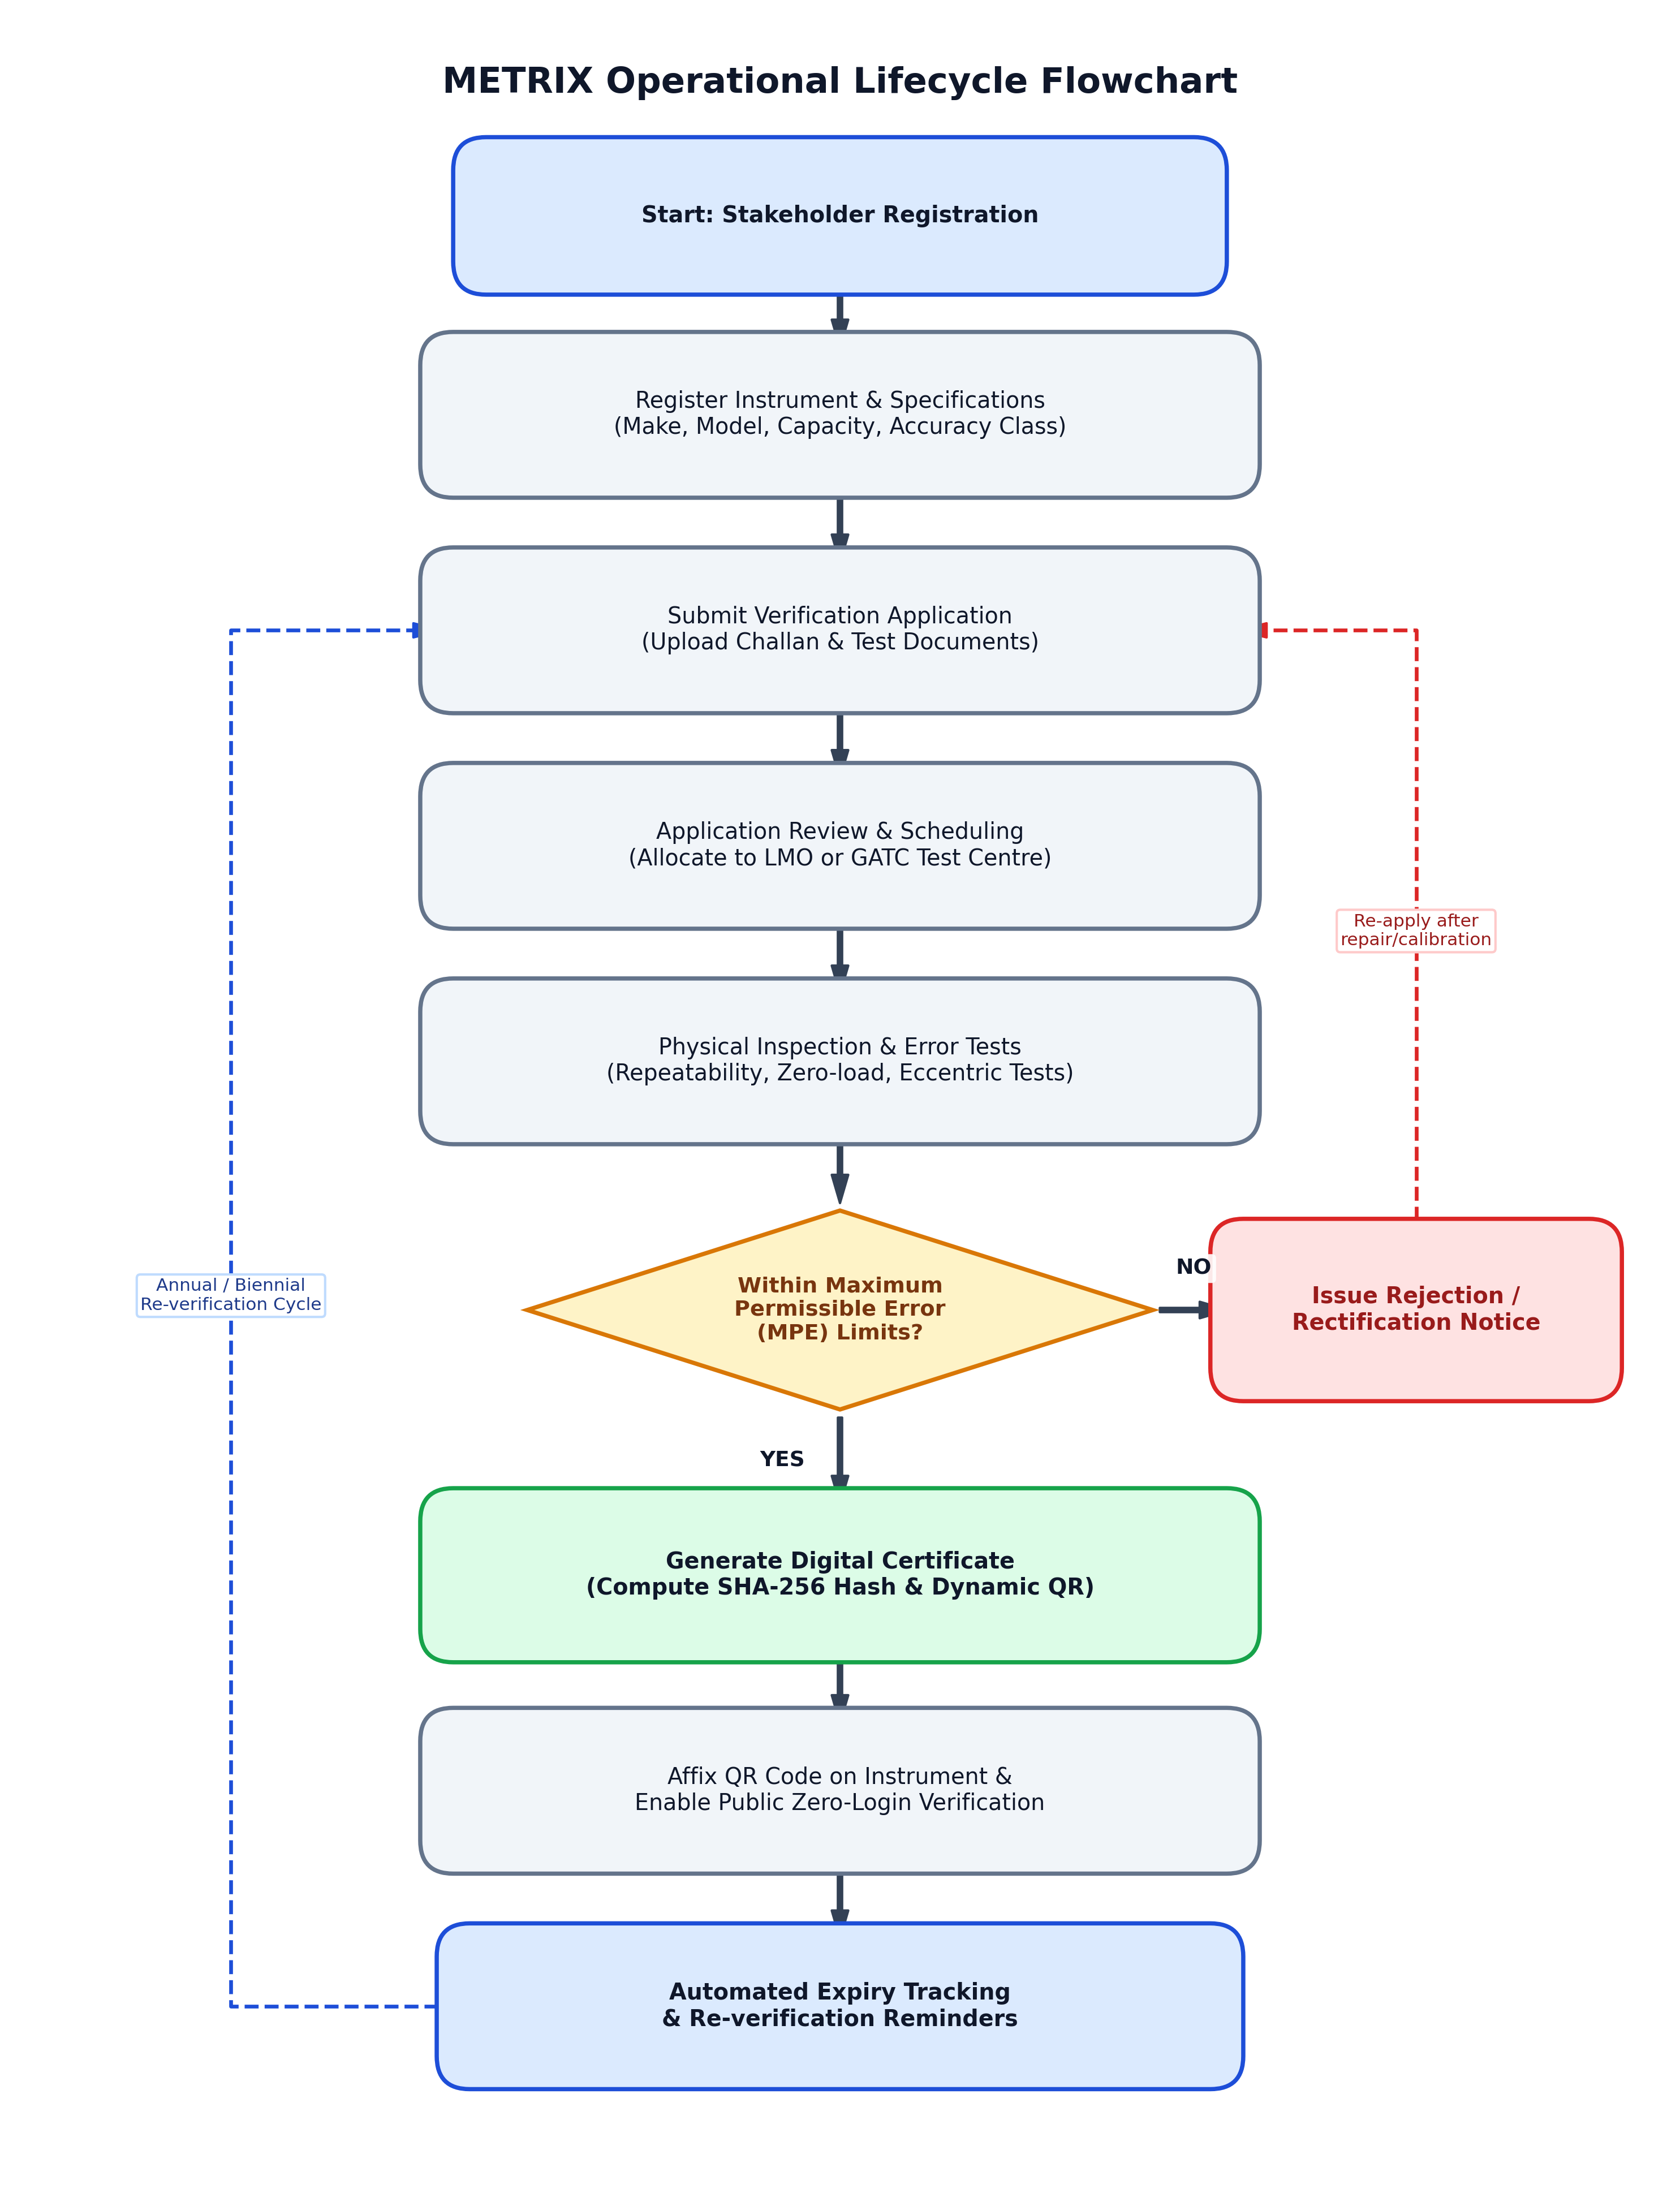
\includegraphics[width=0.82\textwidth]{process_flowchart.png}
\caption{Operational Lifecycle Flowchart of METRIX}
\label{fig:process_flowchart}
\end{figure}


\end{document}
